%%%%%%%%%%%%%%%%%%%%%%%%%%%%%%%%%%%%%%%%%%%%%%%%%%%%%%%%%%%%%%%%%%
% The following comments were written in Portuguese, because this 
% template applies only for School of Technology at University 
% of Campinas, Brazil.
%
% Este é um modelo Latex para monografias de Trabalhos de Conclusão 
% de Curso (TCC) na graduação, monografias de Mestrado e Teses de 
% doutorado da Faculdade de Tecnologia (FT) da Universidade 
% Estadual de Campinas (UNICAMP).
%
% Esse modelo e seu respectivo arquivo de classe de documento 
% foram adaptado do modelo de teses e dissertações do 
% Instituto de Computação da UNICAMP.
%
% Autor: André Leon Sampaio Gradvohl, Dr.
% Email:        gradvohl@ft.unicamp.br
% Lattes CV:    http://lattes.cnpq.br/9343261628675642
% 
% Última versão: 25/setembro/2017
%%%%%%%%%%%%%%%%%%%%%%%%%%%%%%%%%%%%%%%%%%%%%%%%%%%%%%%%%%%%%%%%%%
%
% Escolha: Portugues ou Ingles ou Espanhol.
% Para a versão final do texto, acrescente a palavra "Final",
% como na segunda linha abaixo da próxima.
%\documentclass[Portugues]{tese-FT}
\documentclass[Portugues,Final]{tese-FT}
%\documentclass[Ingles]{tese-FT}
%\documentclass[Espanhol,Final]{tese-FT}

% Para acrescentar comentários ao PDF descomente:
\usepackage
%  [pdfauthor={nome do autor},
%   pdftitle={titulo},
%   pdfkeywords={palavra-chave, palavra-chave},
%   pdfproducer={Latex with hyperref},
%   pdfcreator={pdflatex}]
{hyperref}

%Mantenha o pacote a seguir para citações no formato ABNT
\usepackage[alf]{abntex2cite}

%Mantenha o pacote a seguir para incluir a lista de símbolos.
\usepackage{nomencl}
\makenomenclature

%O pacote a seguir gera um dummy text. Elimine a linha quando
% for editar seu texto.
\usepackage{lipsum}

\begin{document}

% Escolha entre autor ou autora:
\autor{Nome do Autor}
%\autora{Nome da Autora}

% Sempre deve haver um título em português:
\titulo{Título da Dissertação ou Tese em Português}

% Se a língua for o inglês ou o espanhol defina:
%\title{The Dissertation or Thesis Title in English or Spanish for FT}

% Escolha entre orientador ou orientadora e inclua os títulos:
\orientador{Prof. Dr. Nome do Orientador}
%\orientadora{Profa. Dra. Nome da Orientadora}

% Escolha entre coorientador ou coorientadora, se houver, 
% e inclua os títulos:
%\coorientador{Prof. Dr. Eng. Lic. Nome do Co-Orientador}
%\coorientadora{Prof. Dra. Eng. Lic. Nome da Co-Orientadora}

% Escolha entre uma das quatro opções a seguir (comente as demais):
\bsi         % para Trabalho de Conclusão de Curso em BSI
%\tads       % para Trabalho de Conclusão de Curso em TADS
%\qualificacaoMestrado  % Para textos de qualificação de mestrado.
%\qualificacaoDoutorado % Para textos de qualificação de doutorado.
%\mestrado   % para Dissertação de Mestrado em Tecnologia
%\doutorado  % para Tese de Doutorado em Tecnologia

% Se houve cotutela, defina:
%\cotutela{Universidade Nova de Plutão}

%Defina a data da defesa no formato {Dia}{Mês}{Ano}
\datadadefesa{16}{03}{2017}

% Para a versão final defina:
% Repita o nome do Orientador(a) no primeiro avaliador
\avaliadorA{Prof. Dr. Nome do Orientador}{FT/UNICAMP}
\avaliadorB{Profa. Dra. Segunda Avaliadora}{Instituição da segunda avaliadora}
\avaliadorC{Dr. Terceiro Avaliador}{Instituição do terceiro avaliador}
%\avaliadorD{Prof. Dr. Quarto Avaliador}{Instituição do quarto avaliador}
%\avaliadorE{Prof. Dr. Quinto Avaliador}{Instituição do quinto avaliador}
%\avaliadorF{Prof. Dr. Sexto Avaliador}{Instituição do sexto avaliador}
%\avaliadorG{Prof. Dr. Sétimo Avaliador}{Instituição do sétimo avaliador}
%\avaliadorH{Prof. Dr. Oitavo Avaliador}{Instituição do oitavo avaliador}


% Para incluir a ficha catalográfica em PDF na versão final, 
% copie o arquivo PDF, descomente e ajuste a linha a seguir:
%\fichacatalografica{arquivo.pdf}

% Este comando deve ficar aqui:
\paginasiniciais

% Se houver dedicatória, descomente a linha a seguir:
%\prefacesection{Isso é um teste}
%A dedicatória deve ocupar uma única página.
%
%
% Se houver epígrafe, descomente e edite as linhas a seguir:
% \begin{epigrafe}
% {\it
% Vita brevis,\\
% ars longa,\\
% occasio praeceps,\\
% experimentum periculosum,\\
% iudicium difficile.}
%
% \hfill (Hippocrates)
% \end{epigrafe}
%
%
% Agradecimentos ou Acknowledgements ou Agradecimientos
\prefacesection{Agradecimentos}
Os agradecimentos devem ocupar uma única página.

% Sempre deve haver um resumo em português:
\begin{resumo}
O resumo deve ter no máximo 500 palavras e deve ocupar uma única página.
\end{resumo}


% Sempre deve haver um abstract:
\begin{abstract}
The abstract must have at most 500 words and must fit in a single page.
\end{abstract}

% Se houver um resumo em espanhol, descomente as linhas a seguir:
%\begin{resumen}
% A mesma regra aplica-se.
%\end{resumen}

% A lista de figuras:
\listoffigures

% A lista de tabelas:
\listoftables

% A lista de abreviações e siglas é opcional:
% \prefacesection{Lista de Abreviações e Siglas}

% A lista de símbolos é opcional:
% \prefacesection{Lista de Símbolos}

% Quem usa o pacote nomencl para abreviaturas pode incluir:
\renewcommand{\nomname}{Lista de Abreviações e Siglas}
\printnomenclature[3cm]

% O sumário vem aqui:
\tableofcontents

% E esta linha deve ficar bem aqui:
\fimdaspaginasiniciais

% O corpo da dissertação ou tese começa aqui:
%
% O comando a seguir inclui o arquivo introducao.tex
% que contém o capítulo de Introdução. 
% Detalhe: não precisa incluir a extensão .tex
% Aqui começa o capítulo de Introdução.
% Use o comando \label para definir um rótulo, 
% caso seja necessário referenciar esse capítulo
% posteriormente.
\chapter{Introdução}\label{chp:Introducao}

Esse é um texto de exemplo para o modelo de teses e dissertações da Faculdade de Tecnologia (FT) da UNICAMP. Esse modelo se aplica às teses de doutorado, dissertações de mestrado e Trabalhos de Conclusão de Curso, para a graduação (dos cursos de informática da FT).

A seguir, estão alguns exemplos para os elementos mais comuns em textos acadêmicos, \ie tabelas, equações e figuras.

\section{Exemplos de Tabelas e Equações}\label{sec:exemplostabelas}
Aqui um exemplo de como referenciar a \Tabela{tab:tabela_1}. Note que é preciso definir um rótulo (\textit{label}) dentro do comando de definição da tabela.

% Veja a seguir um exemplo de Tabela.
% Você pode usar o site http://www.tablesgenerator.com
% para gerar as tabelas em LaTeX.
\begin{table}[!htp]
\caption[Legenda curta da tabela]{Legenda longa e mais detalhada da tabela.}
\label{tab:tabela_1}
\begin{center}
\begin{tabular}{cc}
\toprule % Linha superior
Coluna 1 & Coluna2 \\ \midrule % Linha do meio 
a & b \\
c & d \\
e & f \\\bottomrule % Linha inferior
\end{tabular}
\end{center}
\end{table}

As tabelas mais complexas podem ser feitas com ajuda no site \href{http://www.tablesgenerator.com}{http://www.tables\-ge\-ne\-ra\-tor.com}.

Veja um exemplo de equação no próprio texto, \eg, $x=\frac{\sqrt{a^{2}+b^{2}}}{\sigma}$.  Se você preferir, pode escrever a equação de forma estendida, conforme a \Equacao{eq:teste} a seguir. Note que o rótulo é colocado automaticamente.

\begin{equation}
x=\frac{\sqrt{a^{2}+b^{2}}}{\sigma}
\label{eq:teste}
\end{equation}

Você também pode obter ajudar para escrever as equações em \LaTeX no site \url{http://www.codecogs.com/latex/eqneditor.php}.

% Note que podemos incluir automaticamente alguns termos na lista de abreviaturas e siglas no pré-texto. Veja exemplos a seguir no código fonte. 

% A sigla \Sigla{abêcê}{ABC} aparecerá automaticamente na lista de abreviaturas e siglas no pré-texto. Do mesmo modo, podemos usar o comando \SiglaHifen{xisipsilonzê}{XYZ} separado por hífen ao invés de aparecer entre parênteses.

Veja na \Secao{sec:exemplo_secao} a seguir como referenciar uma seção. Também será preciso definir um rótulo (\textit{label}) logo após o comando \texttt{\textbackslash section}.

% Aqui começa uma Seção.
% Use o comando \label para definir um rótulo, 
% caso seja necessário referenciar essa seção
% posteriormente.
\section{Exemplo de seção}\label{sec:exemplo_secao} 
Agora observe como se faz uma citação de artigo científico em periódico \cite{Gradvohl2014c}. De acordo com \textcite{Gradvohl2016}, essa é uma citação direta. Se for citar mais de um trabalho, faça da seguinte forma \cite{Caldana2017,Gradvohl2015}. As referências bibliográficas estão no arquivo \texttt{bibliografia.bib}. Outros exemplos de citações também se encontram nesse arquivo.

Veja a seguir o comando para criar uma figura e o resultado, na \Figura{fig:xwing}. Note, no código fonte, que no comando \texttt{caption} podemos estabelecer uma \enquote{legenda curta} para aparecer na Lista de Figuras. A legenda curta é opcional.

\begin{figure}[!htb]
\centering
%As figuras estão na pasta figuras.
% Se seu texto estiver demorando muito para compilar, 
% use figuras no formato PDF ou PNG.
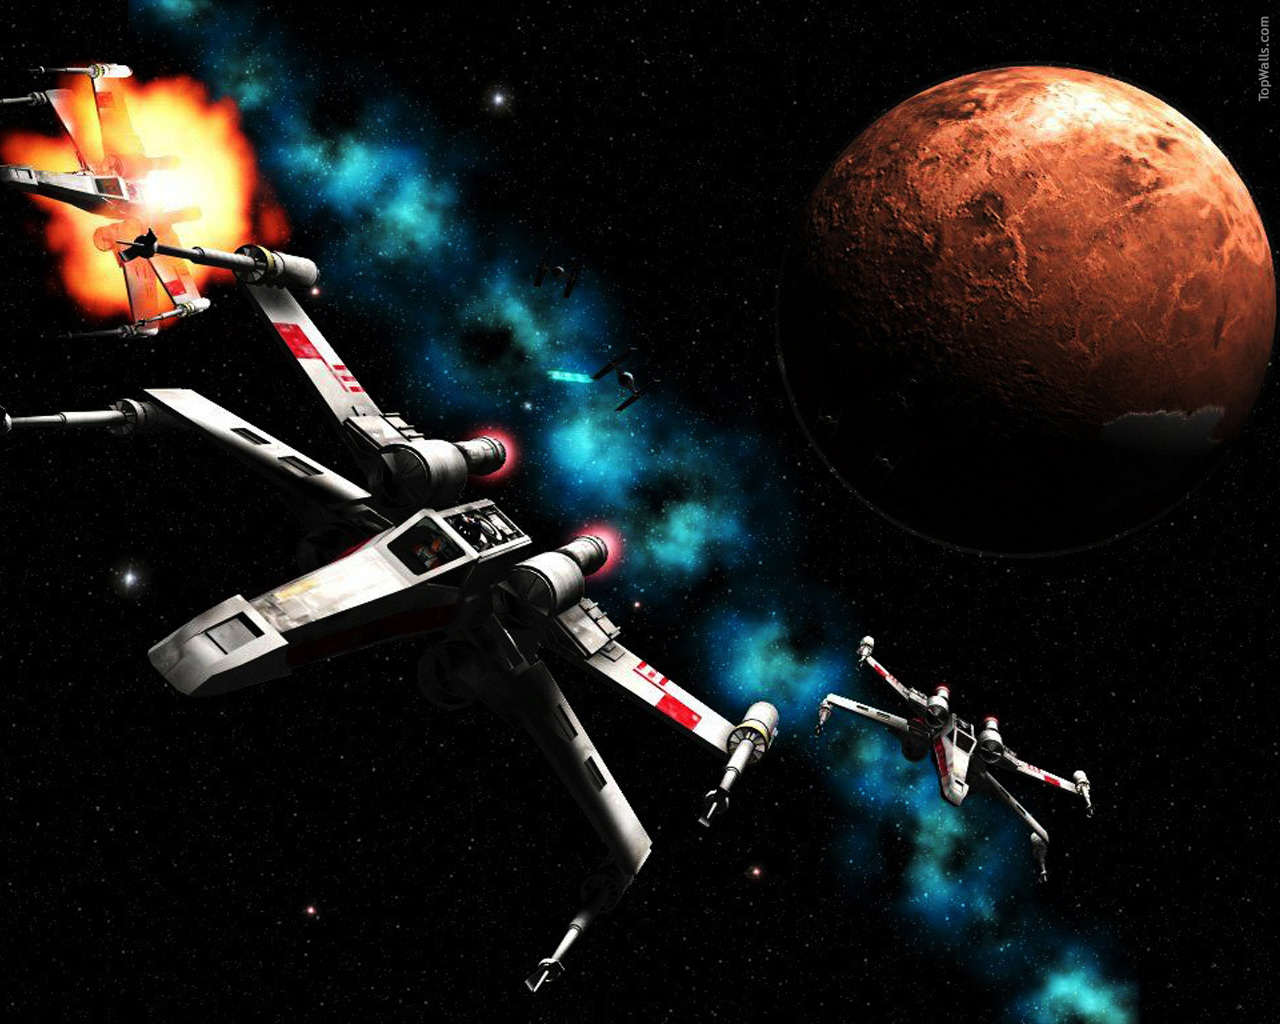
\includegraphics[scale=0.2]{starwars21280.jpg}
\caption[Legenda curta de figura]{Legenda mais extensa de figura.}
\label{fig:xwing}
\end{figure}

Dica importante: sempre que possível, use figuras no formato PDF. De acordo com o Overleaf, isso acelera a compilação do texto, sem perder a qualidade da figura.

\subsection{Exemplo de subseção}
É importante evitar chegar a esse nível de subseção. Dois níveis são suficientes. Use essa opção em último caso, apenas.


\subsection{Exemplo de adição de siglas}\label{subsec:siglas}
Para adicionar uma sigla ou abreviatura na lista de siglas e abreviaturas, use o comando ``\texttt{\textbackslash{}Sigla\{nome por extenso\}\{abreviatura\}}'' ou ``\texttt{\textbackslash{}SiglaHifen\{nome por extenso\}\{abreviatura\}}'' para adicionar a sigla com hífen. 
Por exemplo, respectivamente, \Sigla{Ácido Desoxirribonucleico}{DNA} ou \SiglaHifen{Ácido Ribonucleico}{RNA}. A lista de siglas é adicionada automaticamente.

\section{Comandos opcionais para facilitar}
Este modelo também criou alguns comandos adicionais não apenas para facilitar o trabalho de quem escreve, mas também para manter uma formatação mais consistente.

Entre esses comandos estão o \texttt{\textbackslash{}ie} que inclui a abreviatura ``\ie'' no texto (equivalente ao ``isto é''). Usar esse comando vai garantir que a abreviatura não se separe entre linhas e que o espaço entre o `.' e a próxima letra seja fixo. O mesmo vale para os comandos \texttt{\textbackslash{}eg} que inclui a abreviatura ``\eg'' e \texttt{\textbackslash{}pex} que inclui a abreviatura ``\pex''.

Também existem os comandos \texttt{\textbackslash{}Capitulo\{rótulo do capítulo\}}, \texttt{\textbackslash{}Equacao\{rótulo da equação\}}, \texttt{\textbackslash{}Figura\{rótulo do figura\}}, \texttt{\textbackslash{}Secao\{rótulo da seção\}} e \texttt{\textbackslash{}Tabela\{rótulo da tabela\}}. Esses comandos inserem referências para os respectivos elementos. Além disso, no próprio texto aparece a \textit{string} (``Capítulo'', ``Equação'', ``Figura'' etc) seguida da referência já com o link. Por exemplo, \Secao{sec:exemplo_secao}. Sugere-se a utilização desses comandos para referenciar os respectivos elementos ao invés do comando \texttt{\textbackslash{}ref\{rótulo\}}. Assim, o texto ficará mais uniforme. 

É possível também usar esses comandos nas versões no plurall para conjuntos de referências. Por exemplo, para referenciar várias seções, você pode utilizar o comando \texttt{\textbackslash{}secoes\{rótulo\_1, rótulo\_2, rótulo\_3\}}.

Por exemplo, suponha que queiramos referenciar as \secoes{sec:exemplostabelas,sec:exemplo_secao,subsec:siglas}.

% O comando a seguir inclui o arquivo levantamento.tex
% que contém o capítulo de levantamento bibliográfico. 
% Detalhe: não precisa incluir a extensão .tex
\chapter{Levantamento bibliográfico}\label{chp:levantamento}
% O comando a seguir gera um "dummy text". 
% Elimine-o quando escrever sua dissertação.
\lipsum[6]


% O comando a seguir inclui o arquivo desenvolvimento.tex
% que contém o capítulo de desenvolvimento. 
% Detalhe: não precisa incluir a extensão .tex
\chapter{Desenvolvimento}\label{chp:desenvolvimento}
% O comando a seguir gera um "dummy text". 
% Elimine-o quando escrever sua dissertação.
\lipsum[7]


% O comando a seguir inclui o arquivo conclusoes.tex
% que contém o capítulo de conclusoes. 
% Detalhe: não precisa incluir a extensão .tex
\chapter{Conclusões}\label{chp:conclusoes}
% O comando a seguir gera um "dummy text". 
% Elimine-o quando escrever sua dissertação.
\lipsum[8]


% Os comandos para as referências bibliográficas estão a seguir
% Estilo de bibliografia. Nesse caso é o estilo alfabético.
\bibliographystyle{abntex2-alf}
% As referências bibliográficas estão no arquivo 
% bibliografia.bib . Nesse caso, coloque o arquivo sem a
% extensão .bib.
\bibliography{bibliografia}

% Os anexos, se houver, vêm depois das referências:
\appendix
\chapter{Primeiro Apêndice}
% O comando a seguir gera um "dummy text". 
% Elimine-o quando escrever sua dissertação.
\lipsum[9]

\chapter{Segundo  Apêndice}
% O comando a seguir gera um "dummy text". 
% Elimine-o quando escrever sua dissertação.
\lipsum[10]

\end{document}
